% =====================================================================
%  Physics EE -- detailed structure plan
%  "Investigation on the frequencies of oscillations of a coupled
%   magnetic-mechanical oscillator"
%
%  Compile with pdflatex / xelatex / tectonic (no exotic packages).
%  The figure files referenced in Section 8 live in  figs/  next to this
%  file; comment out the \includegraphics lines if you move the file.
% =====================================================================
\documentclass[11pt,a4paper]{article}

\usepackage[utf8]{inputenc}
\usepackage[T1]{fontenc}
\usepackage[margin=2.2cm]{geometry}
\usepackage{amsmath,amssymb,bm}
\usepackage{booktabs}
\usepackage{array}
\usepackage{longtable}
\usepackage{enumitem}
\usepackage{graphicx}
\usepackage{xcolor}
\usepackage{siunitx}
\usepackage{tcolorbox}
\usepackage[colorlinks=true,linkcolor=blue!60!black,urlcolor=blue!60!black]{hyperref}

\sisetup{separate-uncertainty=true, per-mode=symbol}
\setlist{nosep}
\graphicspath{{figs/}}

% ---- small helpers -------------------------------------------------------
\newcommand{\Y}{Y}                                   % Y = f2^2 - f1^2
\newcommand{\muz}{\mu_0}
\newcommand{\mum}{\mu_m}
\newcommand{\words}[1]{~{\small\color{gray}($\approx$#1 words)}}
\newcommand{\todo}[1]{{\color{red!70!black}\textbf{[#1]}}}
\newtcolorbox{storybox}{colback=blue!4,colframe=blue!50!black,title=Storyline (keep this on your wall)}
\newtcolorbox{notebox}{colback=yellow!8,colframe=orange!70!black,title=Replace with your own values once you have real inputs}

\title{\textbf{Physics Extended Essay -- Detailed Structure Plan}\\[4pt]
\large Investigation on the frequencies of oscillations of a coupled\\ magnetic--mechanical oscillator}
\author{Working document (Edwin's skeleton $+$ INTERNATIONAL's evaluation loop)}
\date{\today}

\begin{document}
\maketitle

\begin{storybox}
Two identical copper leaf springs with repelling magnets form two coupled oscillators.
The in-phase mode ($f_1$) should not feel the magnets; the anti-phase mode ($f_2$) is
stiffened by the magnetic coupling $\gamma$. Modelling the magnets as point dipoles gives
\[
  f_2^2 - f_1^2 \;=\; \frac{3\muz\mum^2}{\pi^3 m\, d^5},
\]
i.e.\ a $-5$ power law. I measured $f_1,f_2$ by video tracking $+$ FFT for
$d = 21$--$60\,$mm. The $\ln$--$\ln$ gradient was $-3.75\pm0.19$, $f_1$ drifted by
2.6\,\%, and points beyond 35\,mm could not be resolved. The evaluation identifies four
systematic effects (FFT resolution/leakage, amplitude-dependent non-linearity of the
$r^{-4}$ force, finite magnet size, non-identical springs). A modified method
(normal-coordinate tracking, longer records, small release, time-domain two-tone
fitting, non-linear least squares) plus an RK4 simulation of the full non-linear
equations quantifies each effect and recovers the dipole law within its range of validity.
\end{storybox}

\tableofcontents
\bigskip

\section{Research question}

\textbf{RQ.} \emph{How does the equilibrium centre-to-centre separation $d$ of the magnets
in a coupled magnetic--mechanical oscillator affect its two normal-mode frequencies $f_1$
and $f_2$, and does the coupling term $f_2^2 - f_1^2$ follow the inverse-fifth-power law
predicted by the magnetic-dipole model?}

Why this wording: it names the independent variable ($d$), the dependent variables
($f_1,f_2$), the derived quantity that is actually tested ($f_2^2-f_1^2$) and the
theoretical claim ($d^{-5}$). Keep the title as it is; put the RQ in \S1.3.

% ---------------------------------------------------------------------------
\section{Mapping: Edwin's structure $\rightarrow$ yours $\rightarrow$ INTERNATIONAL additions}

Word budget is for a 4000-word essay (equations, tables, captions, appendices and
references do not count). If you overrun, shrink 6.1 and 9 first; never shrink
10--13.

\begin{center}\small
\begin{tabular}{@{}p{0.8cm} p{2.9cm} p{6.5cm} r p{3.5cm}@{}}
\toprule
\# & Edwin & Yours (section title) & Words & Extra from INTERNATIONAL \\
\midrule
1 & Introduction 1.1--1.3 & 1.1 Coupled magnetic-mechanical oscillator (done) $\cdot$ 1.2 Modes of oscillation and beats $\cdot$ 1.3 Motivation \& RQ & 350 & motivation paragraph (their \S1.4) \\
2 & Qualitative prediction & 2 Qualitative prediction & 70 & \\
3 & Hypothesis & 3 Hypothesis & 50 & \\
4 & Variable table & 4 Variables (table) & 60 & FFT settings listed as controlled variables \\
9 & Theoretical model (Edwin puts it late) & \textbf{5 Theoretical model} (put it \emph{before} methodology, as INTERNATIONAL does) & 550 & 5.4 ``Remarks on the model'': dimensional check, list of assumptions \\
5--7 & Methodology, data collection, procedures & 6 Methodology: 6.1 FFT background $\cdot$ 6.2 Set-up \& apparatus $\cdot$ 6.3 Method of data collection $\cdot$ 6.4 Procedures & 650 & 6.1 mirrors their \S6.1 (DFT, resolution, leakage, windows) \\
8 & Data & 7 Raw data & 200 & half-range uncertainty and its justification \\
10 & Processed data & 8 Analysis: 8.1 processed table $\cdot$ 8.2 $\ln$--$\ln$ graph $\cdot$ 8.3 $\Y$ vs $d^{-5}$ and $f_1$ vs $d$ $\cdot$ 8.4 comparison with theory & 450 & \\
11 & Discussion \& conclusion & 9 Discussion (preliminary) & 250 & \\
12 & Evaluation & 10 Evaluation: systematic 10.1--10.5, random 10.6 & 550 & each error with sign, size, remedy \\
-- & -- & \textbf{11 Further methodology} & 200 & their \S11 \\
-- & -- & \textbf{12 Further data \& discussion} & 350 & their \S12--13 \\
-- & -- & \textbf{13 Numerical simulation} (RK4) & 300 & their \S14 \\
11.2, 13 & Conclusion, extension & 14 Conclusion \& extensions & 220 & \\
A--E & Appendices & A--H (Section~\ref{sec:appendices}) & 0 & \\
\bottomrule
\end{tabular}
\end{center}

% ---------------------------------------------------------------------------
\section{Section-by-section content}

\subsection*{1 Introduction}
\textbf{1.2 Modes of oscillation and beats.}\words{150}
Same ideas as Edwin's 1.2 but for translational displacements $x_1,x_2$ of the magnets:
in-phase mode ($f_1$: magnets move together, separation constant, magnets ``invisible'');
anti-phase mode ($f_2$: separation oscillates, magnetic force does work). Any release is a
superposition, hence beats with $f_{\rm avg}=(f_1+f_2)/2$ and $f_{\rm beat}=(f_2-f_1)/2$.
Include the identity
\begin{equation}
  4 f_{\rm avg} f_{\rm beat} = f_2^2 - f_1^2 ,
\end{equation}
which ties your test quantity to Edwin's average/beat language and explains why beats
vanish at large $d$ ($f_2\to f_1$). Figure~2: your own sketch of the two modes (do not
copy the IYPT slides). Figure~3: one of your own $x(t)$ traces showing beats.

\textbf{1.3 Motivation \& RQ.}\words{150}
Origin: IYPT 2023 problem~6 ``Magnetic-mechanical oscillator'' (cite the problem
statement); analogy to contactless/magnetically coupled resonators; personal angle
(coupling can be tuned continuously by moving the springs, unlike a fixed spring). State
the RQ.

\subsection*{2 Qualitative prediction \quad 3 Hypothesis}
Repulsion $\propto d^{-4}$, so the stiffness added to the anti-phase mode,
$\gamma=-\mathrm{d}F/\mathrm{d}d\propto d^{-5}$, collapses quickly with $d$: $f_2\to f_1$ and
the beat period $\to\infty$; $f_1$ stays constant.\\
\textbf{Hypothesis:} $f_1$ is independent of $d$; $f_2^2-f_1^2\propto d^{-5}$, i.e.\
$\ln(f_2^2-f_1^2)$ against $\ln d$ is a straight line of gradient $-5$.

\subsection*{4 Variables (table, Edwin style)}
\begin{description}[leftmargin=2.6cm,style=sameline]
\item[Independent] $d$ (centre-to-centre, magnets mounted, measured at equilibrium).
\item[Dependent] $f_1$, $f_2$ (hence $f_2^2-f_1^2$).
\item[Controlled] same spring pair; clamped length $L$; clamp torque; same magnet pair and
orientation; initial displacement (magnitude and which spring); release method; camera
fps, resolution and distance; record length $T$; FFT settings (window, $N$,
zero-padding) -- INTERNATIONAL lists FFT settings as controlled variables, do the same.
\item[Uncontrolled] air currents; temperature ($E$ of copper); residual clamp slip.
\end{description}

\subsection*{5 Theoretical model \words{550}}
\textbf{5.1 Leaf spring as an oscillator.} Cantilever tip stiffness $k=3EI/L^3$;
effective mass $m=M+\tfrac{33}{140}\mu L$ (Rayleigh) so $\omega_0^2=k/m$
(derivation in Appendix~A, or cite). One sentence: the Euler--Bernoulli continuum model of
the IYPT slides reduces to this for a heavy tip mass; a finite-element check shows
$<1\,\%$ difference in $f_2^2-f_1^2$ for $M/(\mu L)\ge0.4$ (numbers in
Section~\ref{sec:numbers}).

\textbf{5.2 Magnetic force.} Coaxial identical dipoles, like poles facing
(from $\bm F=\nabla(\bm\mu\!\cdot\!\bm B)$, Appendix~B):
\begin{equation}
  F(r)=\frac{3\muz\mum^2}{2\pi r^4}\quad\text{(repulsive)} .
\end{equation}
Equilibrium: springs bend outward by $\delta$ with $k\delta=F(d)$. You measure $d$
directly, so the IYPT quintic for the equilibrium point is not needed -- say so.

\textbf{5.3 Linearised coupling and normal modes.}
$F(d+x_2-x_1)\approx F(d)-\gamma\,(x_2-x_1)$ with
\begin{equation}
  \gamma=-F'(d)=\frac{6\muz\mum^2}{\pi d^5}.
\end{equation}
Equations of motion
\begin{equation}
  m\ddot x_1=-kx_1+\gamma(x_2-x_1),\qquad m\ddot x_2=-kx_2-\gamma(x_2-x_1).
\end{equation}
Normal coordinates $\eta=x_1+x_2$, $\xi=x_1-x_2$ (matrix form exactly like Edwin's
eqs.~12--15):
\begin{equation}
  \omega_1^2=\frac{k}{m},\qquad \omega_2^2=\frac{k+2\gamma}{m}
  \quad\Longrightarrow\quad
  \boxed{\,f_2^2-f_1^2=\frac{\gamma}{2\pi^2 m}=\frac{3\muz\mum^2}{\pi^3 m\,d^5}\,}
  \label{eq:main}
\end{equation}
Linearised forms for graphs: (i) $\ln(f_2^2-f_1^2)=\ln C-5\ln d$ with
$C=3\muz\mum^2/(\pi^3 m)$; (ii) $f_2^2-f_1^2=C\,d^{-5}$ (straight line through the origin
against $d^{-5}$; compare its gradient with $C$ from independently measured $\mum$, $m$).

\textbf{5.4 Remarks} (INTERNATIONAL \S5.3 style). Dimensional check
$[\muz\mum^2/(m d^5)]=\si{\per\second\squared}$. List the assumptions you will revisit:
(a) point dipoles, (b) linearised force (small amplitude), (c) identical springs,
(d) lumped mass, (e) no damping, (f) magnets stay coaxial, (g) the FFT returns the true
frequencies.

\subsection*{6 Methodology \words{650}}
\textbf{6.1 FFT background} -- INTERNATIONAL \S6.1 adapted to \emph{frequency} measurement;
the physics you need is in Section~\ref{sec:fft}.\\
\textbf{6.2 Set-up \& apparatus}: labelled photo (Edwin Fig.~3), apparatus list, magnet
specification (grade, $D\times t$, mass), spring dimensions ($L,b,h$), camera (model,
fps, resolution), tracking software.\\
\textbf{6.3 Method of data collection} -- narrate like Edwin \S6: Method~1 (read beat and
average periods from $x(t)$) failed at large $d$ because the envelope disappears when
$f_2-f_1$ is small; Method~2 (FFT of $x(t)$) adopted. Show one $x(t)$ and its FFT with the
two peaks labelled (Edwin Figs.~4--6).\\
\textbf{6.4 Procedures}:
\begin{enumerate}[label=6.4.\arabic*]
\item spring stiffness $k$: static load--deflection, plot $F$ vs $x$, LINEST (Edwin \S7.1);
\item magnet moment $\mum$: either datasheet $B_r$ ($\mum=B_rV/\muz$) or, better, one
magnet on an electronic balance, the other brought coaxially above it at measured $r$,
$F=\Delta m\,g$, fit $F\propto r^{-4}$ (doubles as an independent check of the $r^{-4}$ law);
\item masses $M$, $\mu L$;
\item $f_1,f_2$ vs $d$: set $d$, displace one spring by $A=10$\,mm, release, record $T$\,s
at $f_s$ fps, track, FFT, read the two highest peaks, 3--5 trials per $d$.
\end{enumerate}

\subsection*{7 Raw data \words{200}}
Table~1 basic quantities ($L,b,h,M,\mu,k\pm\Delta k,\mum\pm\Delta\mum,m$). Table~2 $F$ vs
$x$ for $k$. Tables~3/4 $f_1$ and $f_2$ per trial with mean and half-range (justify
half-range vs standard deviation as INTERNATIONAL \S8.2 does: $n=3$--5 is too small for
SD). \textbf{State $T$, $f_s$, $N$ and the bin width $1/T$ in the caption} and add a
column ``resolved? ($f_2-f_1\ge2/T$)''. Rows $d=40$--60\,mm: ``peaks unresolved'' -- this
is a result, not a gap.

\subsection*{8 Analysis \words{450}}
\textbf{8.1} Processed table: $d$, $\ln d\pm\Delta d/d$, $\Y=f_2^2-f_1^2$,
$\Delta\Y=2(f_1\Delta f_1+f_2\Delta f_2)$, $\ln\Y\pm\Delta\Y/\Y$,
$d^{-5}\pm5(\Delta d/d)\,d^{-5}$. One sample calculation (Edwin style).\\
\textbf{8.2} Graph~1: $\ln\Y$ vs $\ln d$ with error bars, best- and worst-fit lines (or
LINEST if the bars are too small). Report the gradient $-3.75\pm0.19$ (unweighted) and
note the weighted value $-3.48\pm0.24$ -- the disagreement itself exposes the
$\ln$-transform problem.\\
\textbf{8.3} Graph~2: $\Y$ vs $d^{-5}$ (theory: straight line through the origin, gradient
$C$). Graph~3: $f_1$ vs $d$ (theory: horizontal) -- you will see the 2.6\,\% drift.\\
\textbf{8.4} Comparison table (Edwin Tables~13/14): theoretical gradient $-5$ (exact) vs
experimental; theoretical $C$ from $\mum,m$ vs the experimental gradient of Graph~2;
percentage differences.

\subsection*{9 Discussion -- preliminary \words{250}}
Trend confirmed ($\Y$ falls steeply, $f_2\to f_1$), but: exponent $-3.75\neq-5$; $f_1$ not
constant; points beyond 35\,mm unresolved; residuals systematic (curvature) rather than
random. Frame the four candidate causes and hand over to \S10.

\subsection*{10 Evaluation \words{550}}
One sub-section per effect, each with \emph{sign, size, remedy}.

\textbf{10.1 FFT resolution \& leakage} (methodological/procedural). Two tones closer than
$\sim1/T$ (rectangular) or $\sim2/T$ (Hann) merge or ``pull'' each other; your
$f_2-f_1=0.039$\,Hz at 35\,mm needs $T\ge26$--51\,s, and 0.009\,Hz at 40\,mm needs
$T\ge110$--220\,s. Show the synthetic-spectrum figure built from \emph{your} $f_1,f_2$
(Fig.~\ref{fig:fft}). Sign: biases the large-$d$ end and flattens the gradient. Remedy
$\to$ \S11.

\textbf{10.2 Non-linear magnetic force} (assumption b). Expand $F(d-\xi)$:
\begin{equation}
  \ddot\xi+\omega_2^2\xi+\alpha\xi^2+\beta\xi^3=0,\qquad
  \alpha=\frac{5}{2}\,\frac{g\,\omega_2^2}{d},\quad \beta=\frac{5\,g\,\omega_2^2}{d^2},\quad
  g=\frac{f_2^2-f_1^2}{f_2^2}.
\end{equation}
Landau--Lifshitz amplitude shift (Appendix~D):
\begin{equation}
  \frac{\Delta\omega}{\omega_2}=\Big(\frac{a}{d}\Big)^2\Big(\frac{15g}{8}-\frac{125g^2}{48}\Big),
  \qquad a=\text{amplitude of }\xi .
\end{equation}
With your $A=10$\,mm release: $+7.6\,\%$ at 21\,mm (RK4 exact: $+9.8\,\%$), $+1.2\,\%$ at
35\,mm (Fig.~\ref{fig:amp}). Sign: $f_2$ overestimated at small $d$, gradient
\emph{steeper} ($-5.16$ in simulation, Fig.~\ref{fig:lnln}) -- a large error but not the
cause of the flattening. Remedy: $A\le3$\,mm, analyse late (small-amplitude) segments,
extrapolate $f_2$ to zero amplitude, RK4 correction (\S13).

\textbf{10.3 Finite magnet size} (assumption a). Replace point dipoles by two uniformly
``charged'' discs per magnet (Gilbert model, Appendix~E). For $d$ only 2--4$\times$ the
magnet diameter the near field is softer than $d^{-5}$: apparent gradient over 21--35\,mm
is $-4.9$ ($D=6$\,mm), $-4.5$ ($D=12$\,mm), $-3.75$ ($D=20$\,mm) (Fig.~\ref{fig:finite};
run \texttt{finite\_size\_magnets.py} with \emph{your} $D,t$). Sign: flattening -- the
leading candidate if your magnets are $\ge12$\,mm. Remedy: exact cylindrical-magnet force
in the model, or larger $d$ (which collides with 10.1 -- discuss the trade-off explicitly).

\textbf{10.4 Non-identical springs} (assumption c) -- analogue of Edwin's 12.2/Appendix~D.
With uncoupled frequencies $f_a\neq f_b$ (Appendix~C):
\begin{equation}
  \omega_{1,2}^2=\bar\omega^2+\kappa\mp\sqrt{\Delta^2+\kappa^2},\qquad
  \kappa=\frac{\gamma}{m},\quad \Delta=\frac{\omega_b^2-\omega_a^2}{2}
  \;\;\Longrightarrow\;\;
  (f_2^2-f_1^2)^2=(f_b^2-f_a^2)^2+(C d^{-5})^2 .
\end{equation}
Consequences: $f_1$ rises as $d$ shrinks (observed $0.802\to0.823$\,Hz; the model with
$f_a=0.793$, $f_b=0.849$\,Hz gives $0.798\to0.819$\,Hz) and $\Y$ saturates at
$|f_b^2-f_a^2|$ instead of $\to0$ -- flattening at large $d$. Remedy: measure $f_a,f_b$
with the other magnet removed; fit the detuned formula.

\textbf{10.5 Damping} (assumption e). Fit the envelope, get $\tau$; frequency shift
$\approx\tfrac12\,(1/4\pi f\tau)^2$ -- negligible for $\tau\sim20$--30\,s -- but the
Lorentzian linewidth $\approx1/(\pi\tau)$ ($\approx0.01$--0.02\,Hz) sets a floor on
resolvability that no record length removes (feeds 10.1). Lumped-mass assumption (d):
$<1\,\%$ (Appendix~A) -- dismiss in one sentence, with the number.

\textbf{10.6 Random errors}: $d$ ($\pm0.5$\,mm, $\Delta(\ln d)=2\,\%$ at 21\,mm), tracking
noise (sub-pixel), frame-timing jitter, release repeatability (half-range across trials),
bin-centring/scalloping $\pm1/(2T)$ unless interpolated.

\subsection*{11 Further methodology \words{200}}
Numbered modified procedure, INTERNATIONAL \S11.2 style:
\begin{enumerate}
\item Measure $f_a,f_b$ of each spring alone (other magnet removed).
\item Track \textbf{both} magnets; form $\eta=x_1+x_2$ and $\xi=x_1-x_2$ \emph{before} the
FFT. Each normal coordinate contains essentially \textbf{one} frequency, so the two-peak
resolution problem disappears -- $f_1$ from $\eta$, $f_2$ from $\xi$, even at 45--60\,mm.
(Physically motivated, free, and the single best improvement.)
\item Record $\ge90$\,s at 60\,fps (or 30\,fps), tripod, scale bar in frame; release
$A\le3$\,mm; also one run at $A=10$\,mm per $d$ for the amplitude study.
\item Re-analyse every record with rectangular / Hann / Blackman windows $+$ 16$\times$
zero-padding $+$ parabolic peak interpolation (INTERNATIONAL Table~10 style comparison),
\textbf{and} with a time-domain two-damped-sinusoid least-squares fit (beats the $1/T$
limit; gives a statistical $\Delta f$).
\item Fit models to $(d,f_1,f_2)$ by weighted non-linear least squares: (a) dipole,
$n=5$; (b) free exponent $n$; (c) finite-size disc model; (d) detuned model. Compare
residuals/$\chi^2$.
\end{enumerate}
\texttt{analyse\_tracks.py} performs steps 4--5 for a folder of Tracker exports.

\subsection*{12 Further data \& discussion \words{350}}
Table: gradient $\pm\Delta$ for each method (rect / Hann / Blackman / two-tone fit /
normal-coordinate FFT) -- like INTERNATIONAL Figs.~26--27. Graph: $f_2$ vs amplitude
(segments) with extrapolation to zero amplitude. Graph: $\ln\Y$ vs $\ln d$ for old vs new
data with both theory curves (point dipole and finite size). Discuss which correction
moved the gradient toward $-5$ and by how much; be explicit if a residual discrepancy
remains and what it implies (e.g.\ ``the dipole law is valid only for $d\gtrsim4D$'').

\subsection*{13 Numerical simulation \words{300}}
RK4 integration of the \textbf{full} equations
\begin{equation}
  m\ddot x_1=-kx_1-\big[F(d+x_2-x_1)-F(d)\big],\qquad
  m\ddot x_2=-kx_2+\big[F(d+x_2-x_1)-F(d)\big],\qquad F=C_F r^{-4},
\end{equation}
(optionally with the finite-size $F$) using your measured $k,m,C_F$. Two uses:
(i) predict $f_2(A,d)$ $\to$ the amplitude correction used in \S12;
(ii) generate synthetic $x(t)$ at your fps and $T$ and push them through the \emph{same}
FFT pipeline $\to$ isolates the bias caused purely by the analysis (in my test at
$T=40$\,s, window peak-picking gave gradients $-3.3$ to $-3.5$ while the two-tone fit
recovered the true value). Code $\to$ Appendix~G.

\subsection*{14 Conclusion \& extensions \words{220}}
Answer the RQ in three sentences ($f_1$ constant within \ldots; $f_2^2-f_1^2$ falls as
$d^{-n}$ with $n=\ldots\pm\ldots$; the dipole law holds for $d\ge\ldots$). Name the
dominant systematic error and what fixed it. Extensions: vary $\mum$ (magnet grade) at
fixed $d$ to test the $\mum^2$ dependence; attractive orientation (softening $\to$
instability at a critical $d$); three springs; eddy-current damping with a copper plate.

% ---------------------------------------------------------------------------
\section{FFT error analysis -- what to write}\label{sec:fft}

INTERNATIONAL needed \textbf{amplitudes} (SNR), so its corrections were energy-correction
factors and baseline-noise subtraction. You need \textbf{frequencies}, so the relevant FFT
physics is different -- say this explicitly.

\begin{enumerate}
\item \textbf{Resolution.} $X_k=\sum_{n=0}^{N-1}x_n e^{-2\pi i kn/N}$; bin spacing
$\Delta f_{\rm bin}=f_s/N=1/T$. Two tones are separable only if $|f_2-f_1|\gtrsim1/T$
(rectangular) or $\gtrsim2/T$ (Hann; main lobe twice as wide). From your data:

\begin{center}\small
\begin{tabular}{@{}S[table-format=2.0] S[table-format=1.3] S[table-format=1.1] S[table-format=3.0] S[table-format=3.0]@{}}
\toprule
{$d$/mm} & {$f_2-f_1$/Hz} & {bins at $T=20$\,s} & {$T_{\min}$ rect/s} & {$T_{\min}$ Hann/s}\\
\midrule
21 & 0.240 & 4.8 & 4 & 8\\
25 & 0.141 & 2.8 & 7 & 14\\
28 & 0.097 & 1.9 & 10 & 21\\
31 & 0.074 & 1.5 & 14 & 27\\
35 & 0.039 & 0.8 & 26 & 51\\
40 & 0.009 & 0.2 & 111 & 222\\
\bottomrule
\end{tabular}
\end{center}

\item \textbf{Leakage \& windows.} Rectangular: narrowest main lobe (best for two close
peaks of similar height) but $-13$\,dB side lobes; Hann: 4-bin main lobe, $-31$\,dB;
Blackman: 6-bin, $-58$\,dB. Because both your peaks have similar amplitude and there is no
strong interferer, the rectangular (or Hann) window is the right choice -- the opposite of
the usual ``Hann by default'' advice, and unlike INTERNATIONAL's case. Amplitude
correction factors are \textbf{not} needed because you only read peak positions.
\item \textbf{Peak pulling.} When main lobes overlap the two maxima are pushed apart or
merge; in my synthetic test ($T=20$\,s) the errors were $\pm2$--7\,mHz at 21--31\,mm,
$\pm10$\,mHz at 35\,mm and total failure at 40\,mm -- quote your own numbers from
\texttt{ee\_simulations.py} Part~A with your real $T$ and $f_s$.
\item \textbf{Scalloping / bin-centring.} The true frequency lies anywhere within
$\pm\tfrac12$\,bin, i.e.\ $\pm1/(2T)$, unless you zero-pad and interpolate (parabola
through the three bins around the peak). Zero-padding interpolates the spectrum, it does
\emph{not} add resolution -- make that distinction.
\item \textbf{Damping linewidth.} $e^{-t/\tau}\cos(2\pi ft)$ has FWHM $\approx1/(\pi\tau)$;
with $\tau\approx25$\,s that is 0.013\,Hz -- comparable to $f_2-f_1$ at 40\,mm, so beyond
$\sim35$\,mm the modes cannot be separated by any spectral method applied to a single
coordinate $\to$ justification for normal-coordinate tracking and time-domain fitting.
\item \textbf{Sampling.} $f_s=$ fps (30/60\,Hz) $\gg2f$, no aliasing; but video frame timing
jitters and frames drop $\to$ resample to a uniform grid before the FFT (the script reports
the jitter).
\item \textbf{Propagation into your graph.}
$\Delta(\ln\Y)=2(f_1\Delta f_1+f_2\Delta f_2)/\Y$ grows from 0.04 to 1.1 across your range
for $\Delta f=5$\,mHz, so error bars must be drawn in $\ln$-space and the fit weighted;
otherwise the noisy large-$d$ points dominate the gradient.
\end{enumerate}

% ---------------------------------------------------------------------------
\section{``Non-linearisation'' improvements -- three levels (use all three, in order)}

\begin{description}[style=nextline]
\item[Level 1 -- analysis (cheap, do it now).] Replace ``take logs then LINEST'' with a
weighted non-linear least-squares fit of $\Y=C d^{-n}$ (and $\Y=Cd^{-5}$ with $n$ fixed) to
the un-transformed data. Advantages to state: no point is discarded because $\ln(0)$ or
$\ln(\text{negative})$ fails; heteroscedastic errors are handled by the weights; $C$ and
$n$ come with proper uncertainties. With your 6 points: $n=3.5\pm0.2$ (vs $\ln$--$\ln$
$-3.75$) -- report both and explain the difference.
\item[Level 2 -- physics (the systematic-error story).] The model linearised $F(r)$ about
$d$. Keep the full $r^{-4}$ (or finite-size) force: perturbation formula (Appendix~D) in
the body, RK4 (\S13) for exact numbers, amplitude-segment analysis $+$ extrapolation to
$A\to0$ for the data. Tabulate the size of the correction at each $d$.
\item[Level 3 -- model (finite size $+$ detuning).] Fit models (c) and (d) of \S11
step~5. Present the comparison of residual patterns as the decisive evidence for which
assumption failed.
\end{description}

% ---------------------------------------------------------------------------
\section{Lab / data checklist (you have lab access and the raw tracks)}

\begin{itemize}[label=$\square$]
\item Magnet dimensions $D,t$, mass $M$, grade ($B_r$) -- needed for \S10.3 and the theoretical $C$.
\item Spring $L,b,h,\mu$ (weigh a known length), $k$ by static loading; $f_a,f_b$ of each spring alone.
\item Balance measurement of $F(r)$ for 4--6 values of $r$ (checks $r^{-4}$ and gives $\mum$).
\item Re-run $d=21\ldots60$\,mm with both magnets tracked, $T\ge90$\,s, $A=3$\,mm (and one
$A=10$\,mm run each). Name files \texttt{d21\_trial1.csv} etc.
\item \texttt{python analyse\_tracks.py \textquotedbl tracks/*.csv\textquotedbl{} -\/-out results} $\to$ per-file
diagnostic figure ($x(t)$ $+$ two-tone fit, three-window FFT, $f_2$ vs amplitude),
\texttt{summary.csv}, and the $\ln$--$\ln$ gradient per method. Then form $\eta,\xi$ from
the two tracked magnets and run the same script on them.
\item Sanity check of magnitudes: $\gamma=2\pi^2 m\Y$ from your data vs
$\gamma=6\muz\mum^2/(\pi d^5)$ from $\mum$. If they differ by more than a factor $\sim2$,
revisit the coaxial-dipole assumption or the definition of $d$ before writing \S8.4.
\item Re-derive the $f_2-f_1$ requirement with your real $T$: if your original records were
$\sim20$--40\,s, say in \S7 that 35\,mm was marginal and 40\,mm unresolvable.
\end{itemize}

% ---------------------------------------------------------------------------
\section{Figures and tables (final list)}

\textbf{Figures:} 1 set-up sketch (done) $\cdot$ 2 mode sketch $\cdot$ 3 set-up photo
$\cdot$ 4 $x(t)$ with beats (small $d$) $\cdot$ 5 $x(t)$ with no visible envelope (large
$d$) $\cdot$ 6 FFT with two peaks $\cdot$ 7 $F$ vs $x$ ($k$) $\cdot$ 8 $F$ vs $r$ on the
balance ($\mum$) $\cdot$ 9 $\ln\Y$ vs $\ln d$ (Graph~1) $\cdot$ 10 $\Y$ vs $d^{-5}$
(Graph~2) $\cdot$ 11 $f_1$ vs $d$ (Graph~3) $\cdot$ 12 synthetic-spectrum resolution
figure $\cdot$ 13 $f_2$ vs amplitude $\cdot$ 14 gradient by method (further data) $\cdot$
15 old vs new data with dipole and finite-size theory $\cdot$ 16 RK4 vs linearised
prediction.

\textbf{Tables:} 1 constants $\cdot$ 2 $k$ data $\cdot$ 3/4 $f_1,f_2$ raw $\cdot$ 5
processed $\cdot$ 6 theory vs experiment (gradient, $C$) $\cdot$ 7 systematic-error summary
(effect, sign, size, remedy) $\cdot$ 8 further raw data (appendix) $\cdot$ 9 gradient/$C$
per method and per model $\cdot$ 10 simulated vs measured $f_2$ shift.

% ---------------------------------------------------------------------------
\section{Supporting figures already generated}

\begin{figure}[htbp]\centering
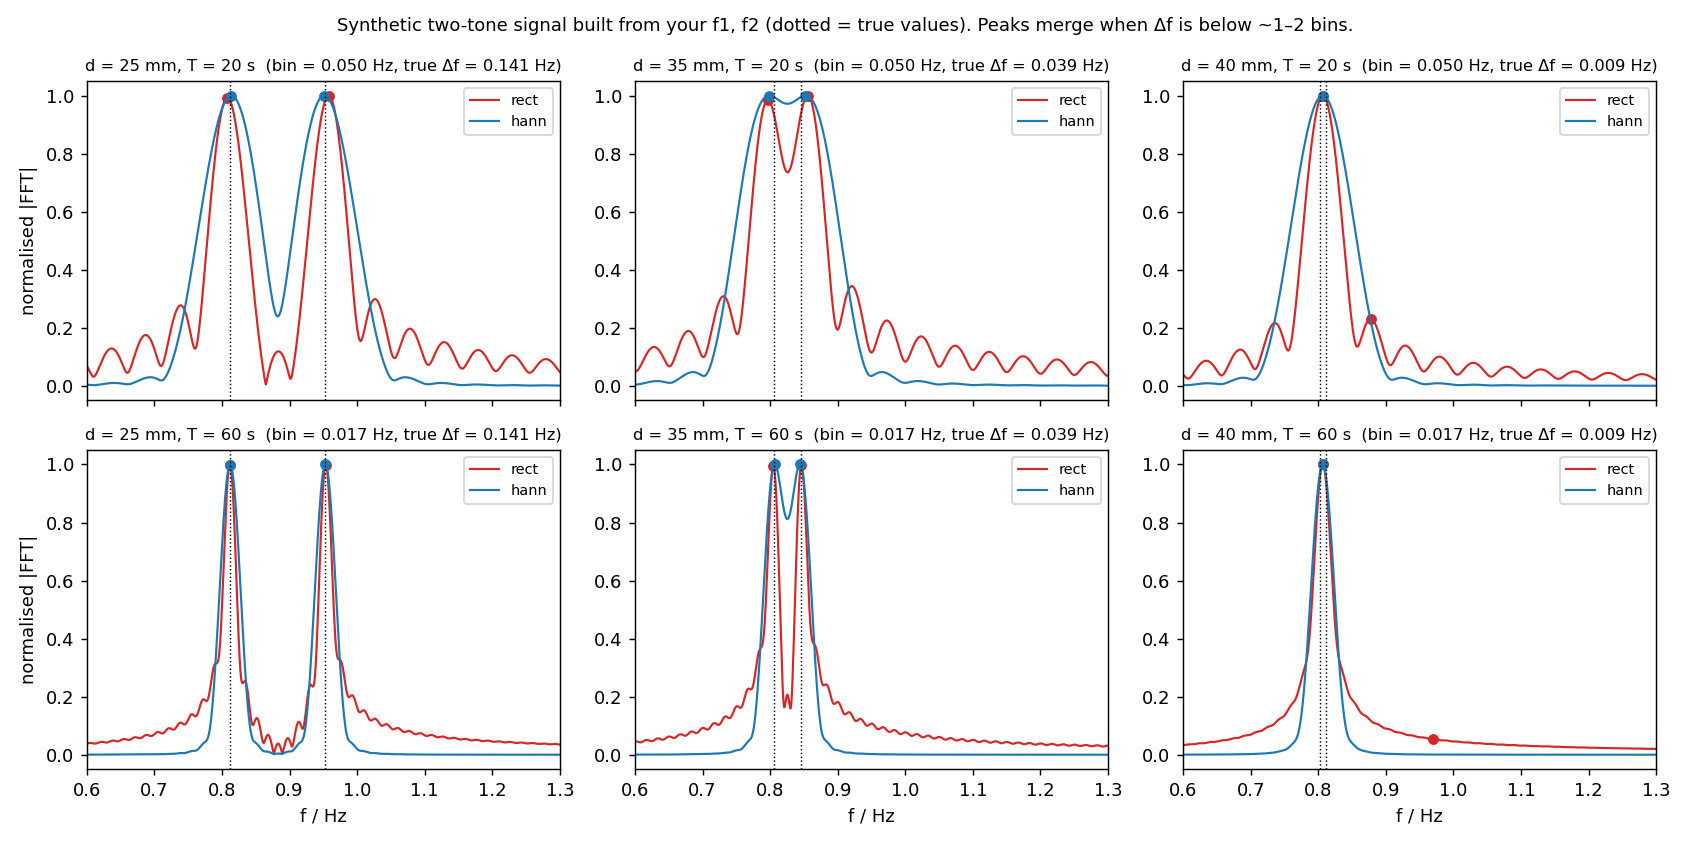
\includegraphics[width=\textwidth]{A_fft_resolution.png}
\caption{Synthetic two-tone spectra built from your $f_1,f_2$ (dotted lines $=$ true
values) for $T=20$\,s and 60\,s. Peaks merge when $f_2-f_1$ falls below $\sim$1--2 bins.
\emph{Use in \S10.1.}}\label{fig:fft}
\end{figure}

\begin{figure}[htbp]\centering
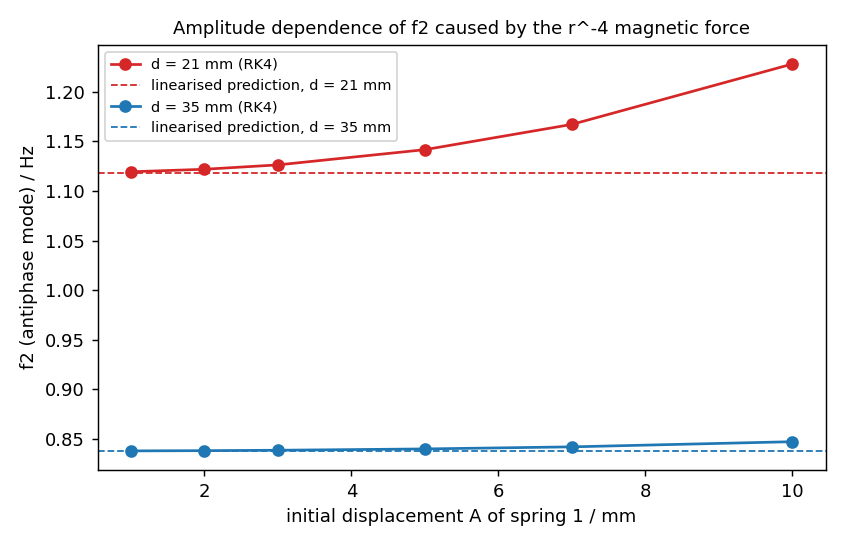
\includegraphics[width=0.62\textwidth]{B_f2_vs_amplitude.png}
\caption{RK4 simulation: amplitude dependence of $f_2$ caused by the $r^{-4}$ force,
compared with the linearised prediction. \emph{Use in \S10.2 / \S13.}}\label{fig:amp}
\end{figure}

\begin{figure}[htbp]\centering
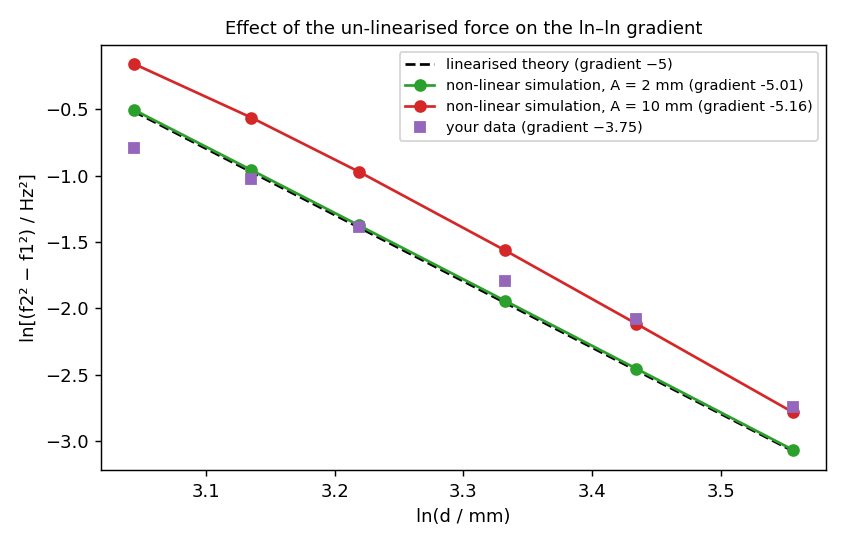
\includegraphics[width=0.62\textwidth]{B_lnln_gradient.png}
\caption{Effect of the un-linearised force on the $\ln$--$\ln$ gradient: linearised theory
($-5$), non-linear simulation at $A=2$ and 10\,mm, and your data.
\emph{Use in \S10.2.}}\label{fig:lnln}
\end{figure}

\begin{figure}[htbp]\centering
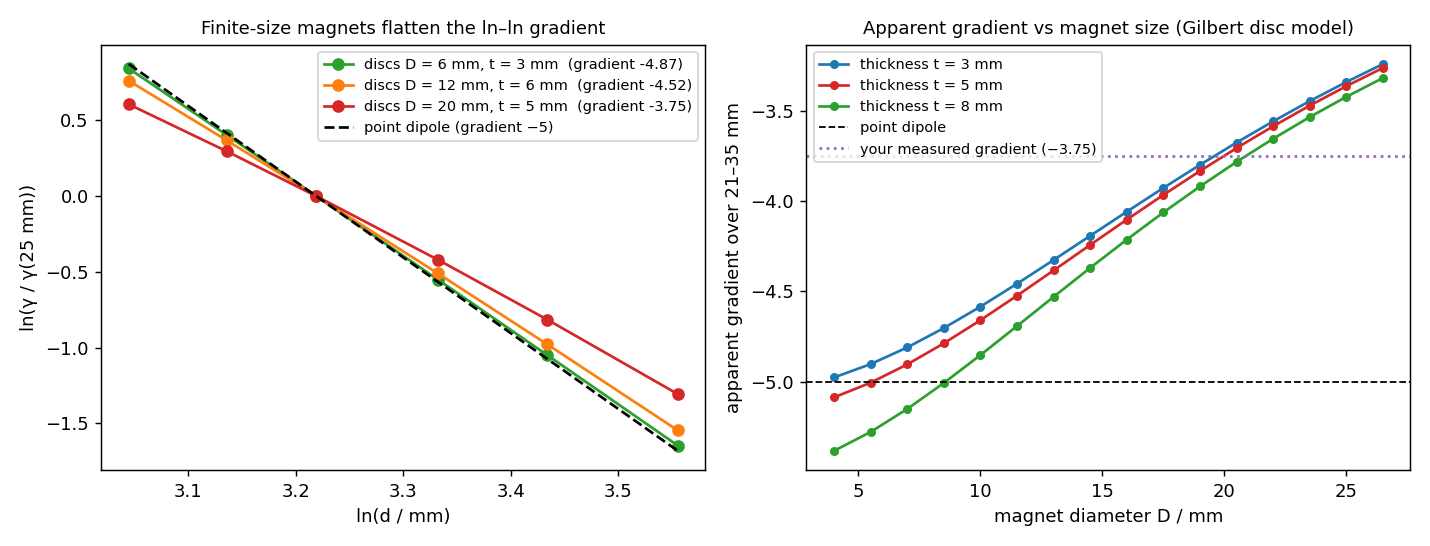
\includegraphics[width=\textwidth]{D_finite_size_gradient.png}
\caption{Finite-size (charged-disc) magnet model: apparent $\ln$--$\ln$ gradient over
21--35\,mm versus magnet diameter and thickness. \emph{Use in \S10.3.}}\label{fig:finite}
\end{figure}

\begin{figure}[htbp]\centering
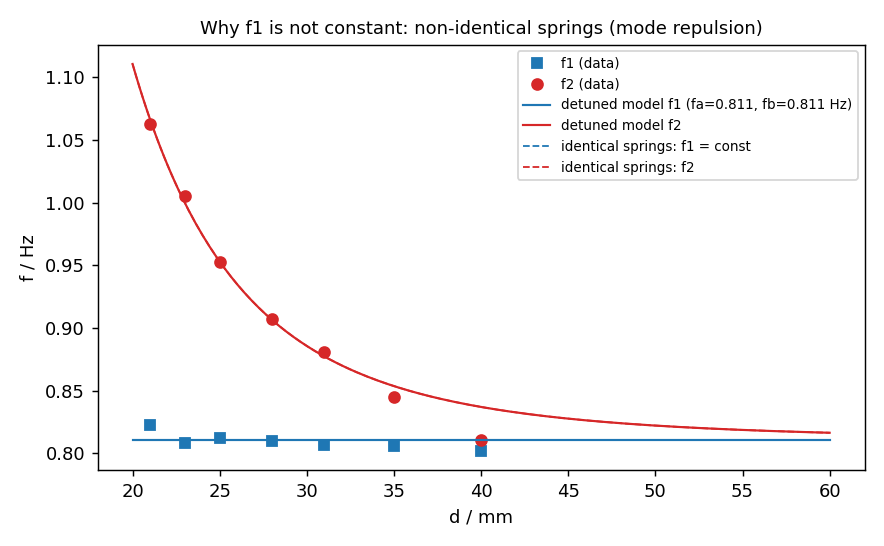
\includegraphics[width=0.62\textwidth]{E_detuning.png}
\caption{Why $f_1$ is not constant: detuned (non-identical springs) model versus the
identical-spring model. \emph{Use in \S10.4.}}\label{fig:detune}
\end{figure}

\clearpage
% ---------------------------------------------------------------------------
\section{Appendices to write}\label{sec:appendices}

\begin{description}[leftmargin=1.2cm,style=nextline]
\item[A] Cantilever stiffness $3EI/L^3$, effective mass $\tfrac{33}{140}\mu L$, and FEM
check of lumped vs beam model ($<1\,\%$).
\item[B] Dipole field $\to$ force between coaxial dipoles $F=3\muz\mum^2/(2\pi r^4)$
$\to$ $\gamma=6\muz\mum^2/(\pi d^5)$.
\item[C] Detuned normal modes $\omega_{1,2}^2=\bar\omega^2+\kappa\mp\sqrt{\Delta^2+\kappa^2}$
and the $d^{-5}$ limit.
\item[D] Series expansion of $F(d-\xi)$, $\alpha$ and $\beta$, Landau--Lifshitz amplitude
shift $(a/d)^2(15g/8-125g^2/48)$, comparison with RK4.
\item[E] Finite-size (charged-disc) magnet force and apparent-gradient table.
\item[F] Uncertainty propagation ($\Delta\Y$, $\Delta\ln\Y$, $\Delta d^{-5}$, LINEST worst
lines).
\item[G] Python: \texttt{analyse\_tracks.py} (FFT windows, two-tone fit, segments),
\texttt{ee\_simulations.py} (RK4, synthetic FFT), \texttt{finite\_size\_magnets.py}.
\item[H] Further raw data tables (all windows/methods), as INTERNATIONAL Appendix~A.
\end{description}

% ---------------------------------------------------------------------------
\section{Ready-made numbers from my checks}\label{sec:numbers}

\begin{notebox}
\emph{Assumed in the scripts:} $f_s$, $\tau$, magnet size and mass -- marked \texttt{\# ASSUMED}.
\begin{itemize}
\item $\ln$--$\ln$ fit, 6 points: gradient $-3.75\pm0.19$, intercept 10.68 (matches your
chart); weighted ($\Delta f=5$\,mHz): $-3.48\pm0.24$. Free power law on raw $\Y$:
$n=3.5\pm0.2$.
\item Non-linear force, $A=10$\,mm release: $f_2$ $+9.8\,\%$ (21\,mm), $+1.1\,\%$
(35\,mm); gradient $-5.00\to-5.16$. $A=2$\,mm: $+0.3\,\%$ / $+0.03\,\%$.
\item Finite-size discs, apparent gradient over 21--35\,mm: $D=6$\,mm $-4.87$ $\cdot$
10\,mm $-4.6$ $\cdot$ 12\,mm $-4.5$ $\cdot$ 15\,mm $-4.2$ $\cdot$ 20\,mm $-3.75$ $\cdot$
25\,mm $-3.4$ ($t=3$--6\,mm changes these by $<0.1$).
\item Lumped vs beam: $\Y$ differs by 0.03\,\% ($M/\mu L=3.3$), 0.4\,\% (0.8), 1\,\% (0.4).
\item Detuned model fitted with $n=5$: $f_a=0.793$\,Hz, $f_b=0.849$\,Hz reproduces the
$f_1$ drift $0.798\to0.819$\,Hz.
\item Synthetic tracks at $T=40$\,s: window peak-picking gradients $-3.3$ to $-3.5$;
two-tone fit $-4.9$ (true $-4.9$) $\to$ the analysis method alone can shift the gradient
by more than 1.
\end{itemize}
\end{notebox}

% ---------------------------------------------------------------------------
\section{Pitfalls to avoid (examiner's eye)}
\begin{itemize}
\item Do not present the 40\,mm point as data; present the unresolved range as a measured
limit of the method.
\item Do not claim ``$f_1$ constant'' when it drifts 2.6\,\%; explain it (10.4).
\item Do not copy IYPT slide figures or equations without derivation; cite the IYPT
problem and derive the lumped model yourself.
\item Keep all corrections quantitative (sign and size) -- hand-waving loses evaluation marks.
\item Every graph: error bars, best/worst lines or LINEST uncertainty, units, gradient with
uncertainty, theory line overlaid where possible.
\item Word count: equations, tables, captions, appendices excluded -- move derivations
there ruthlessly.
\end{itemize}

\end{document}
